\chapter{Przebieg badań}
Doświadczenie polegało na analizie porównawczej sprawności algorytmów opisanych w \refsource{rozdziale}{cha:dos} w \refsource{sekcji}{sec:alg}. Celem doświadczenia było określenie jakości algorytmu utworzonego w ramach pracy inżynierskiej autora\cite{Blyszcz2022}. Szczegółowa metodologia badawcza została określona w \refsource{podrozdziale}{sec:met}.

\section{Metodologia badawcza}
\label{sec:met}
Przyjęta w projekcie metodologia badawcza została określona w poniższej \refsource{tabeli}{tab:met-bad}. Przyjęta metodologia ma za zadanie określić jakoś porównywanego algorytmu.

\begin{table}[H]
    \centering
    \captionsource{Metodologia badawcza}{Opracowanie własne}
    \begin{tabular}{|L{\textwidth}|}
        \hline
        \textbf{Problem badawczy:} \\
        Czy algorytm klasyfikacji danych utworzony w ramach pracy inżynierskiej może konkurować z rozwiązaniami dostępnymi w środowiskach komercyjnych \\ \hline

        \textbf{Pytania badawcze:} \\
        \begin{enumerate}
            \item Czy algorytm jest konkurencyjny pod względem wybranych metry:
            \begin{itemize}
                \item dokładność algorytmu
                \item czas działania
                \item precyzja
                \item czułość
                \item f1
                \item auc
            \end{itemize}
        \end{enumerate} \\ \hline

        \textbf{Hipotezy:} \\
        \begin{enumerate}
            \item Nie ma istotnej różnicy w uzyskanej ''\textit{dokładności}'' między algorytmami.
            \item Nie ma istotnej różnicy w uzyskanej ''\textit{czułości}'' między algorytmami.
            \item Nie ma istotnej różnicy w uzyskanej ''\textit{precyzji}'' między algorytmami.
            \item Nie ma istotnej różnicy w uzyskanym ''\textit{auc}'' między algorytmami.
            \item Nie ma istotnej różnicy w uzyskanej ''\textit{f1}'' między algorytmami.
            \item Nie ma istotnej różnicy w uzyskanym ''\textit{czasie działania}'' między algorytmami.
        \end{enumerate} \\ \hline
    \end{tabular}
    \label{tab:met-bad}
\end{table}

\section{Przygotowanie platformy}
Do badań wykorzystano narzędzie ''\textit{Projektant}'' znajdujące się na platformie ''\textit{Azure Machine Learning Studio}'' (Azure ML). Narzędzie to umożliwiło utworzenie interaktywnego potoku zadań. Potok ten składa się z kilku części:
\begin{itemize}
    \item Przygotowanie i obróbka zbiorów danych
    \item Trenowanie oraz testowanie algorytmów klasyfikacji danych
    \item Utworzenie tabeli porównawczej dla wyników poszczególnych algorytmów (\refsource{obraz}{fig:pipeline}).
\end{itemize}

\subsection{Przygotowanie danych}
W pierwszym kroku dane zostały znormalizowane za pomocą metody \textbf{MinMax}, która przekształca dane numeryczne do wartości w zakresie ${0, 1}$. W następnym kroku za pomocą języka Python oraz biblioteką Pandas oraz Numpy zostają zamienione etykiety słowne na wartości \textbf{0} i \textbf{1} oraz następuje zamiana wartości $[NaN, -inf, inf]$ na cyfrę $0$. Cały proces został zobrazowany na \refsource{diagramie}{fig:norm}

\begin{figure}[H]
    \centering
    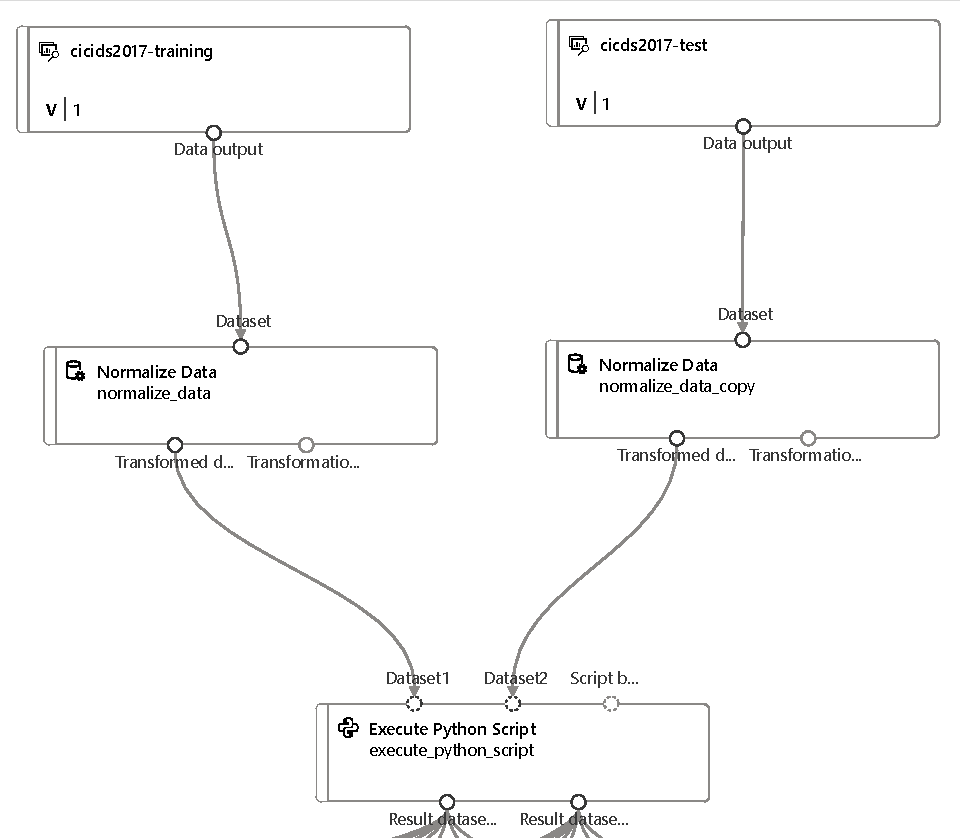
\includegraphics[width=0.6\textwidth]{images/norm}
    \captionsource{Potok normalizacji danych}{Opracowanie własne}
    \label{fig:norm}
\end{figure}

\subsection{Trenowanie oraz testowanie algorytmów}
Kolejną grupą zadań widoczną w potoku są te związane z trenowaniem i testowaniem poszczególnych algorytmów opisanych w \refsource{rozdziale}{cha:dos}. Każdy test składa się 3 kafelek. W przypadku algorytmów dostarczonych wraz z platformą Azure ML są to:
\begin{itemize}
    \item \textbf{model klasyfikujący} - odpowiada za przygotowanie algorytmu klasyfikacyjnego
    \item \textbf{blok treningowy} - tworzy wytrenowany model, za pomocą połączonego zbioru danych
    \item \textbf{blok ewaluacyjny} - sprawdza wcześniej wytrenowany model za pomocą powiązanego zbioru danych.
\end{itemize}
Potok zadań wykorzystujący algorytmy dostarczone przez Microsoft Azure został ukazany na \refsource{schemacie}{fig:ms-pipe}

\begin{figure}[H]
    \centering
    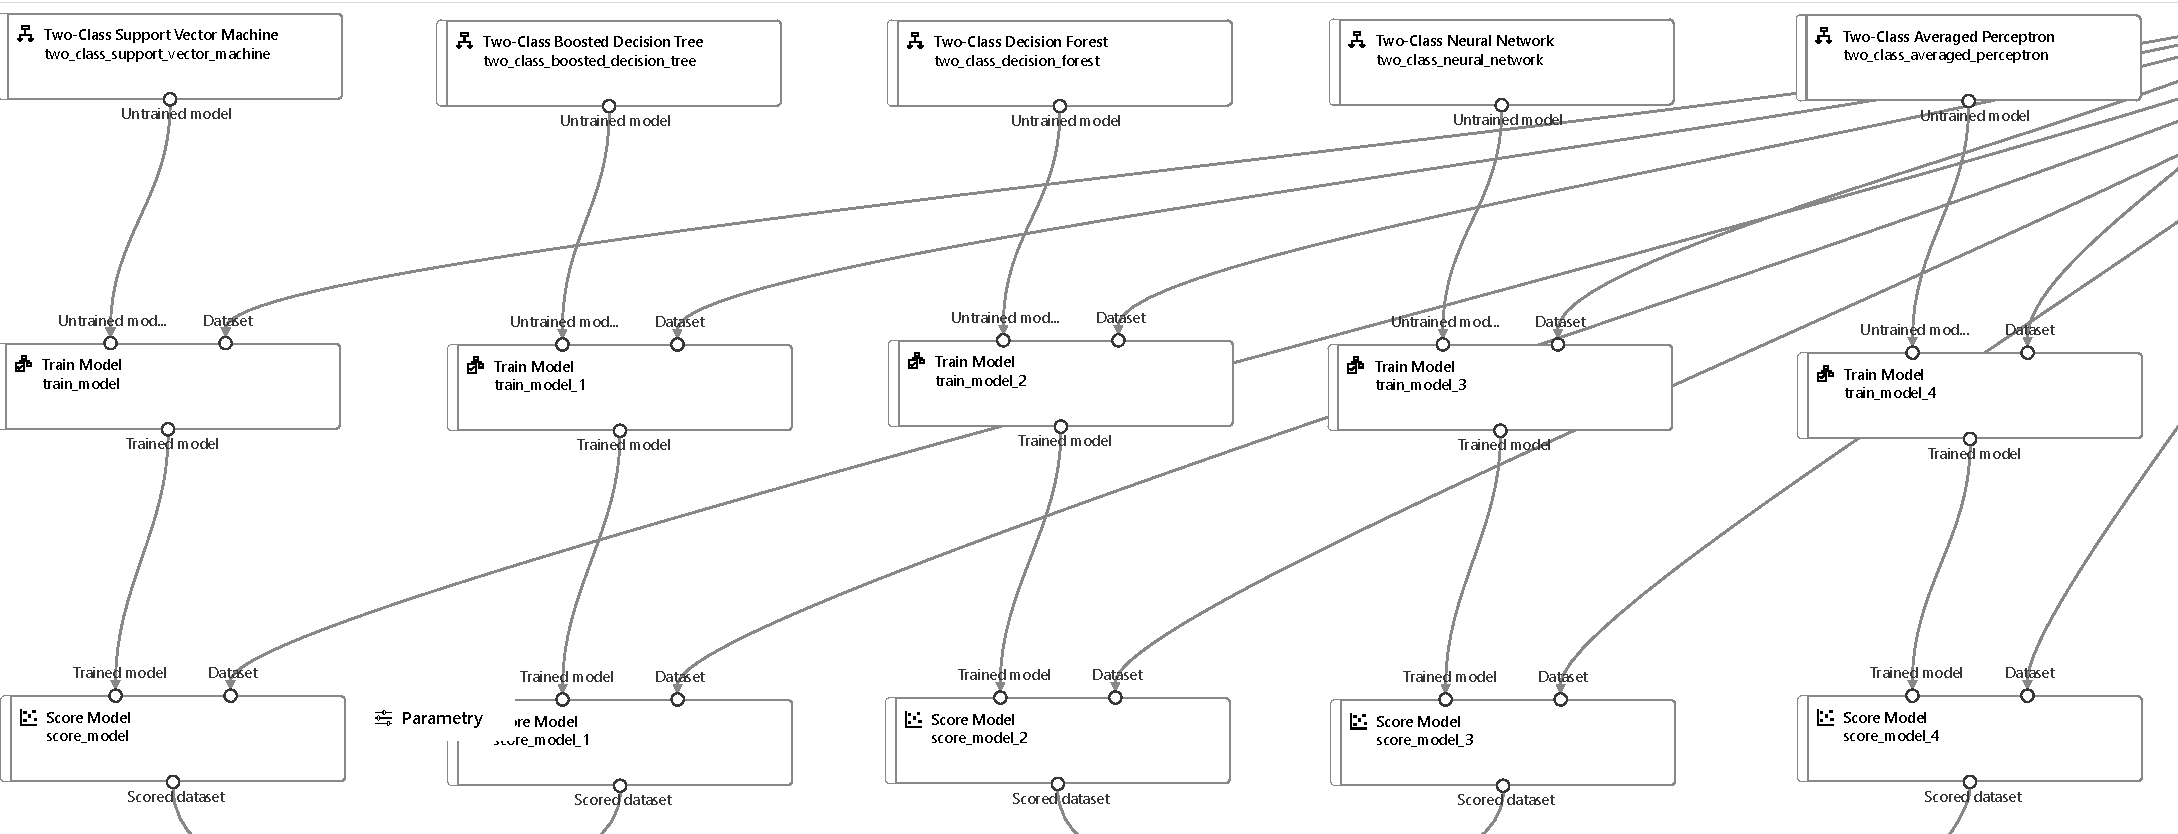
\includegraphics[width=\textwidth]{images/ms_pipe}
    \captionsource{Potok zadań dla algorytmów klasyfikacyjnych}{Opracowanie własne}
    \label{fig:ms-pipe}
\end{figure}

Algorytmy dostarczone w ramach pracy badawczej składają się z:
\begin{itemize}
    \item \textbf{biblioteka Python} - archiwum o rozszerzeniu \textbf{.zip}, które zawiera w sobie odpowiednie pliki napisane w języku Python
    \item \textbf{blok treningowy} - wykorzystuje dostarczoną bibliotekę do wytrenowania modelu oraz zapisania na platformie Azure najlepszego uzyskanego wyniku za pomocą powiązanego zbioru danych
    \item \textbf{blok ewaluacyjny} - wykorzystuje dostarczoną bibliotekę do ewaluacji algorytmu za pomocą połączonego zbioru danych
\end{itemize}

Potok zadań dla algorytmów niestandardowych został ukazany na \refsource{rysunku}{fig:au-pipe}

\begin{figure}[H]
    \centering
    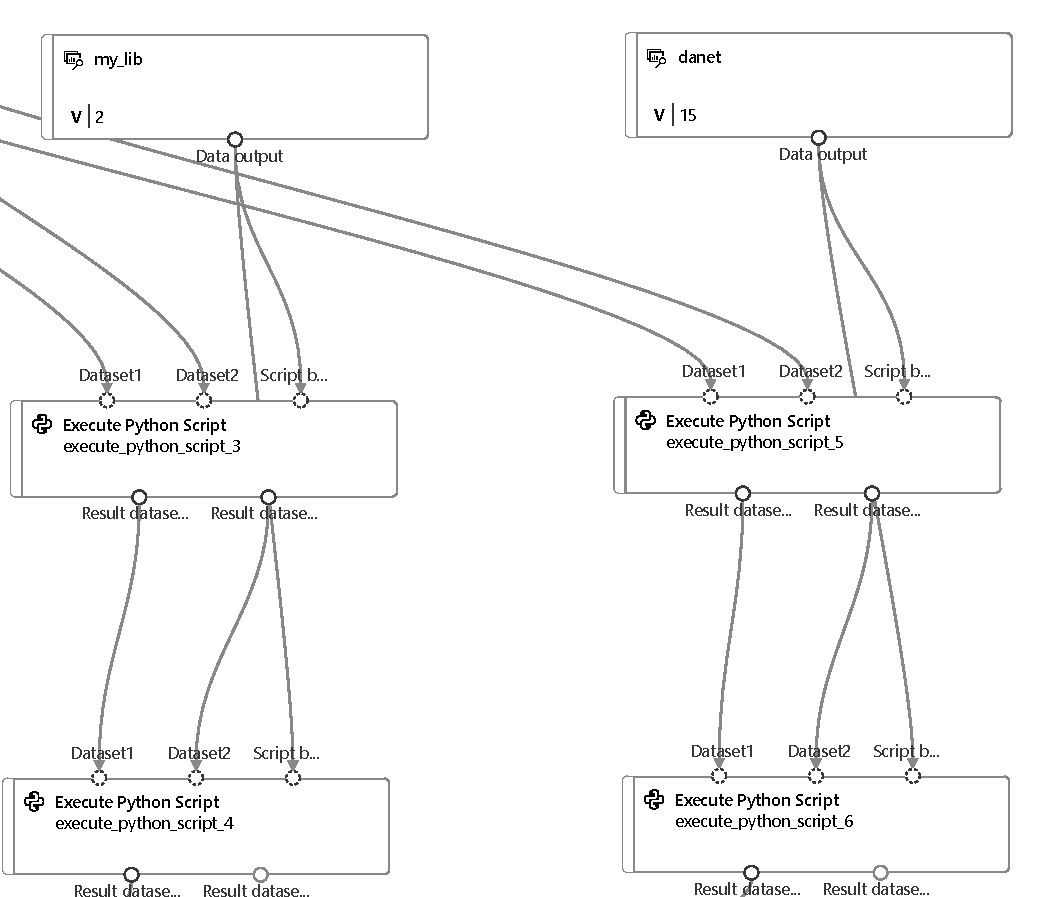
\includegraphics[width=0.8\textwidth]{images/au-pipe}
    \captionsource{Potok zadań dla algorytmów klasyfikacyjnych}{Opracowanie własne}
    \label{fig:au-pipe}
\end{figure}


\subsection{Utworzenie tabeli porównawczej}
Kolejną częścią zadań jest zebranie wyników poszczególnych algorytmów oraz połączenie ich w jedną całość. Wykorzystano do tego moduły języka Pyton, które zwracają przetwożone wyniki oraz łączą je w jedną tabelę zbiorczą, co pokazano na \refsource{rysunku}{fig:pipe-4}.

\begin{figure}[H]
    \centering
    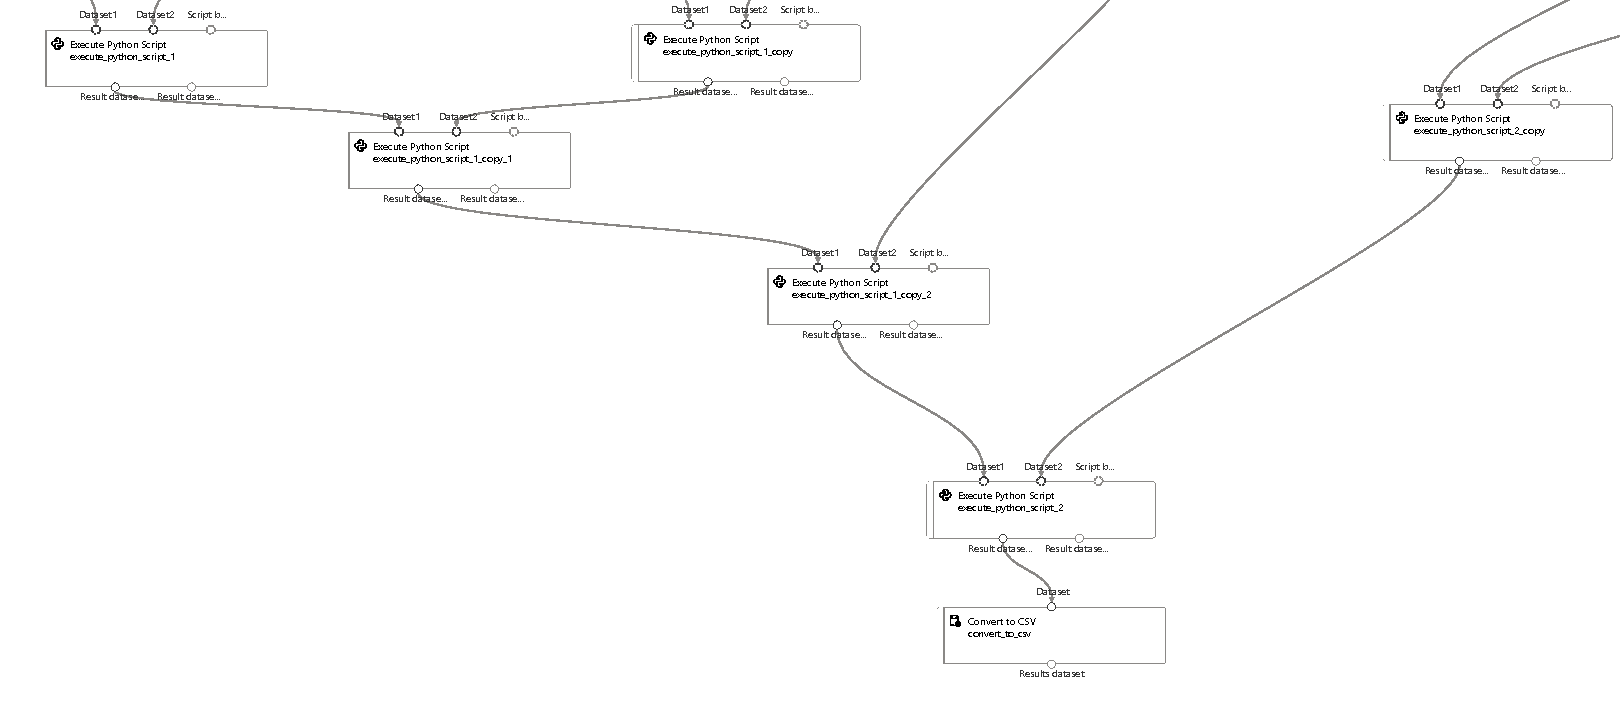
\includegraphics[width=\textwidth]{images/pipe-csv}
    \captionsource{Moduły odpowiedzialne za przetwożenie wyników}{Opracowanie własne}
    \label{fig:pipe-4}
\end{figure}

\section{Weryfikacja potoku}

\begin{landscape}
    \vspace*{\fill}
    \begin{figure}[H]
        \centering
        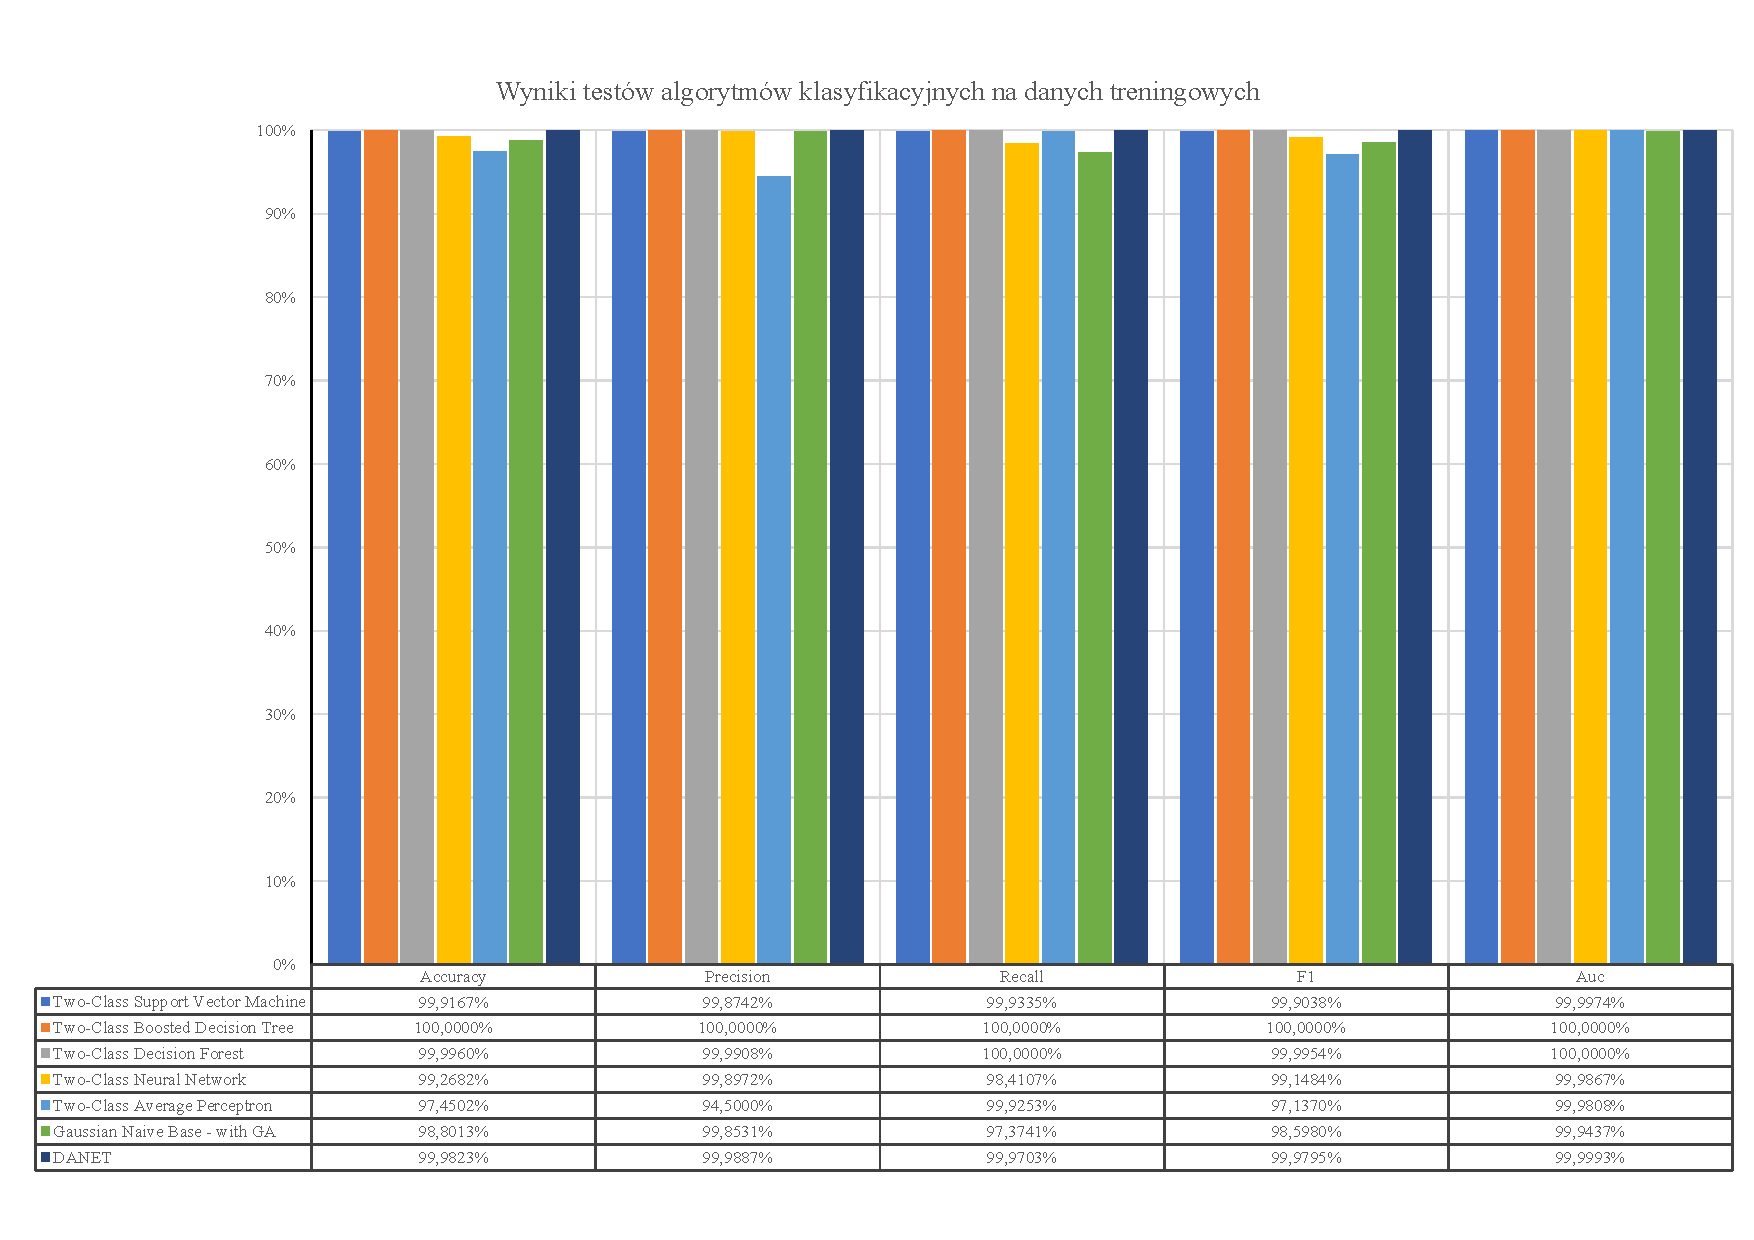
\includegraphics[height=0.8\textwidth]{images/predict_same}
        \captionsource{Wyniki testów algorytmów klasyfikacyjnych na danych treningowych}{Opracowanie własne}
        \label{fig:predict-same}
    \end{figure}
\vfill

\end{landscape}

\section{Próba badawcza}

\begin{landscape}
    \vspace*{\fill}
    \begin{figure}[H]
        \centering
        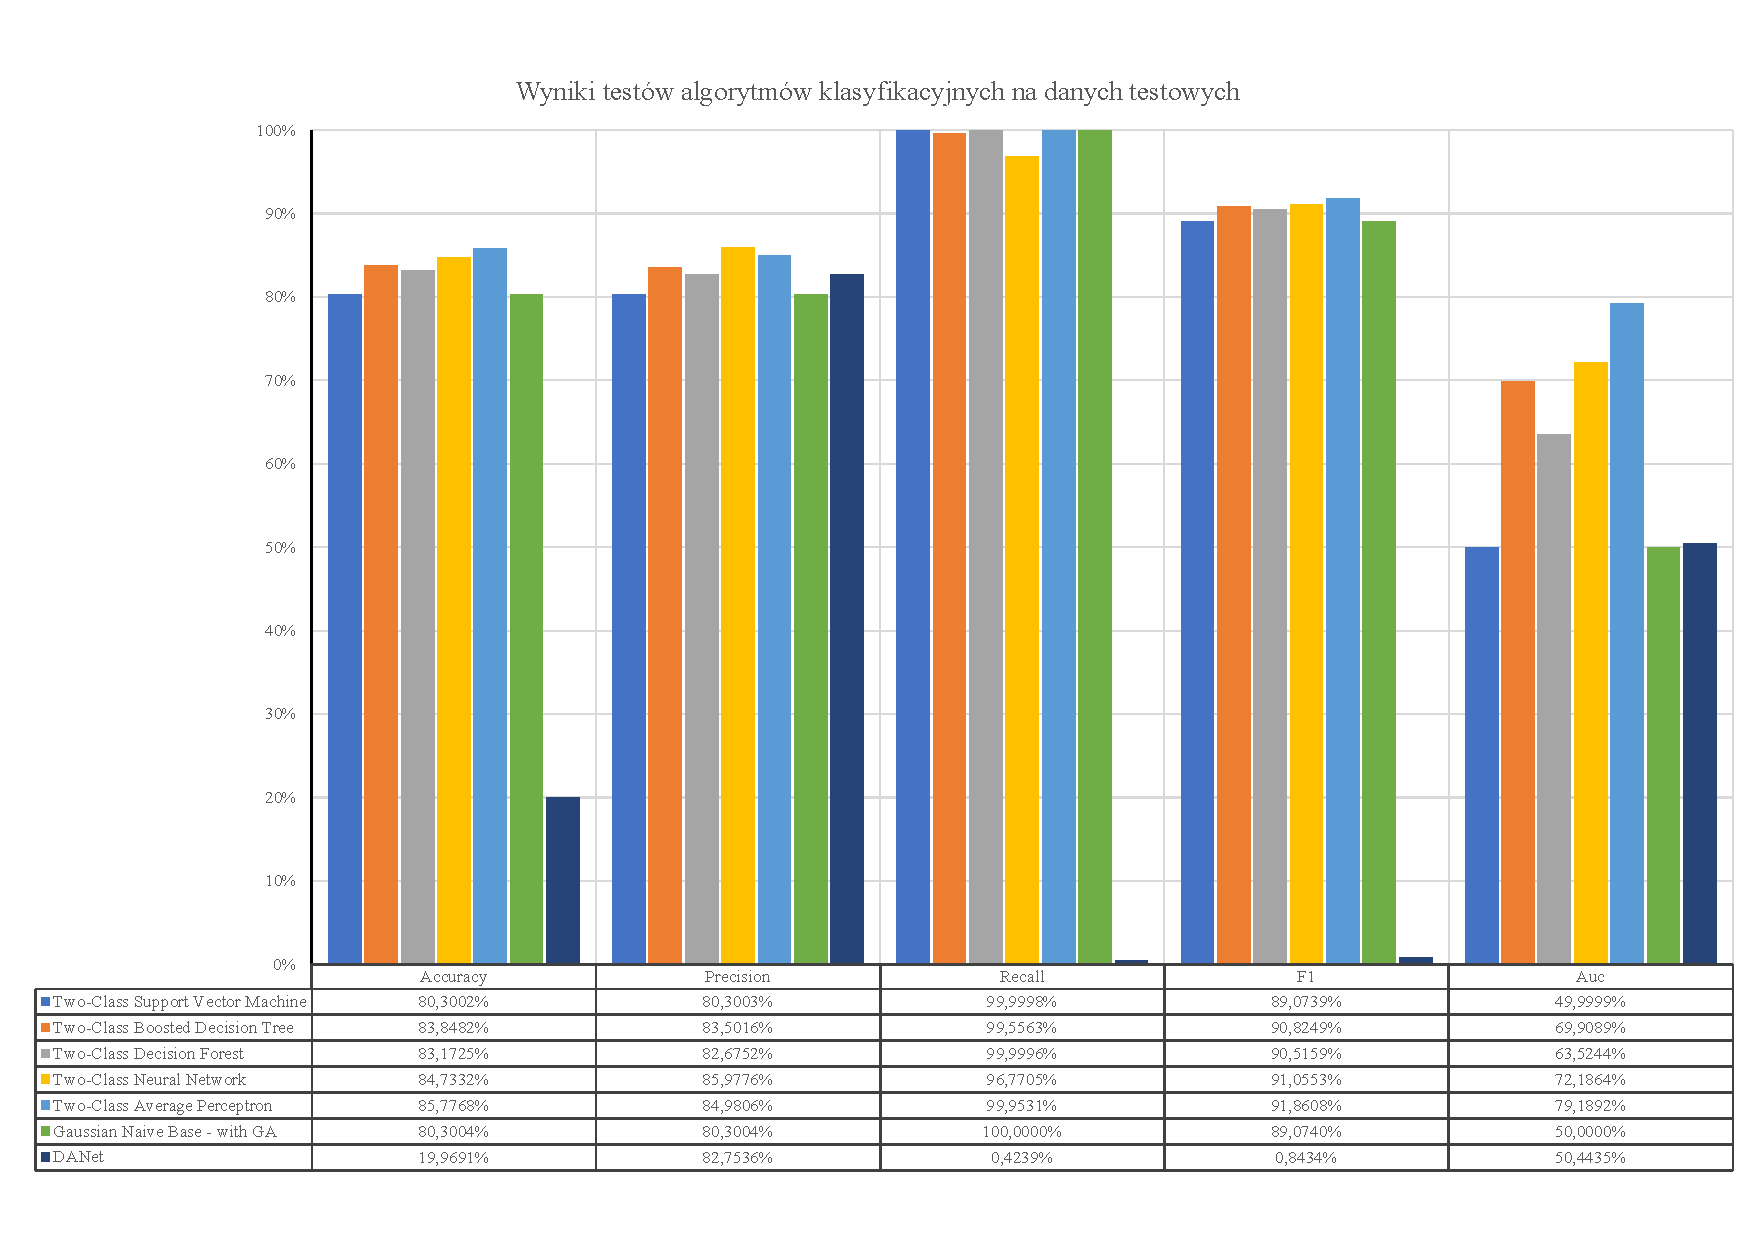
\includegraphics[height=0.8\textwidth]{images/predict_result}
        \captionsource{Wyniki testów algorytmów klasyfikacyjnych na danych testowych}{Opracowanie własne}
        \label{fig:predict-result}
    \end{figure}
    \vfill
\end{landscape}


\section{Wnioski}

